\documentclass{beamer}

\usepackage[T1]{fontenc}
\usepackage[utf8]{inputenc}
\usepackage[english]{babel}

\usepackage{graphicx}
\usepackage{animate}

\usepackage{listings}
\lstset{ %
    language=C,
    basicstyle=\footnotesize,
    morekeywords={__kernel,__global,__local,uint}
}

\usepackage[numbers]{natbib}
\bibliographystyle{plainnat}

\begin{document}

\title{A* GPGPU Implementations for Path-Finding}
\author{Florian Klemme}
\frame{\titlepage}

\begin{frame}
    \frametitle{Overview}
    \tableofcontents
\end{frame}

\section{The A* search algorithm}
\subsection{The basics}
\begin{frame}
    \frametitle{The A* search algorithm}
    \begin{columns}
        \column{0.6\textwidth}
        %\animategraphics[autoplay, width=1.2\textwidth]{5}{AstarProgressAnimation/astar-}{0}{194}
        \includegraphics[height=1.2\textwidth]{AstarProgressAnimation/astar-194}
        
        \column{0.4\textwidth}
        \begin{itemize}
            \item \textbf{A*} is a \emph{best-first search} algorithm
            \item Chooses minimal node \(f(n) = g(n) + h(n)\)
            \item Needs \emph{priority queue} to select next node
            \item Needs look-up data structure for visited nodes
        \end{itemize}
        
        \vspace{1em}
        Animation CC~BY~3.0 Subh83 on wikimedia.org
    \end{columns}
\end{frame}

\subsection{GPGPU approaches}
\begin{frame}
    \frametitle{Multi-agent A* vs. parallel GA*}
    Problem: It's hard to parallelize the priority queue!
    
    \vspace{1em}
    \begin{columns}[T]
        \column{0.5\textwidth}
        \textbf{Multi-agent A*}~\cite{silva2011gpu}
        \begin{itemize}
            \item Per-agent local priority queue
            \item Node and edge information can be shared. Open and closed list has to be stored for each agent.
            \item \textbf{Local memory is a scarce resource!} I've seen 16, 32~and 48~kilobyte.
        \end{itemize}
        
        \column{0.5\textwidth}
        \textbf{Parallel GA*}~\cite{zhou2015massively}
        \begin{itemize}
            \item Multiple independent priority queues
            \item Expand multiple nodes at the same time
            \item The challenge is \textbf{handling of duplicate nodes!}
            \item Again, bound by memory
        \end{itemize}
    \end{columns}
\end{frame}

\section{Priority queue as binary heap}
\subsection{Dispatch memory access}
\begin{frame}[fragile]
    \frametitle{Priority queue: Dispatch memory access}
    \begin{lstlisting}
typedef struct {
    __local  uint_float *localMem;
    const    size_t      localSize;
    __global uint_float *globalExt;
             size_t      size;
} OpenList;

uint_float _read_heap(OpenList *open, size_t index) {
    return index < open->localSize ?
        open->localMem[index] :
        open->globalExt[index - open->localSize];
}

void _write_heap(OpenList *open, size_t     index,
                                 uint_float value) {
    if (index < open->localSize)
        open->localMem[index] = value;
    else
        open->globalExt[index - open->localSize] = value;
}
    \end{lstlisting}
\end{frame}

\subsection{Binary heap functions}
\begin{frame}[fragile]
    \frametitle{Priority queue as binary heap}
    \begin{columns}[T]
        \column{0.5\textwidth}
        We need the common\dots
        \begin{itemize}
            \item push
            \item top \& pop
        \end{itemize}
    
        \column{0.5\textwidth}
        But also\dots
        \begin{itemize}
            \item find
            \item update
        \end{itemize}
    \end{columns}
    
    \vspace{1em}
    \begin{lstlisting}
void push(OpenList *open, uint value, float cost) {
    _push_impl(open, &open->size, value, cost);
}

void update(OpenList *open, size_t index, uint  value,
                                          float cost) {
    _push_impl(open, &index, value, cost);
}
    \end{lstlisting}
\end{frame}

\subsection{Push, pop and find}
\begin{frame}[fragile]
    \frametitle{Binary heap: Push}
    \begin{lstlisting}
void _push_impl(OpenList *open,  size_t *size,
                uint      value, float   cost) {
    size_t index = (*size)++;

    while (index > 0) {
        size_t parent = (index - 1) / 2;

        uint_float pValue = _read_heap(open, parent);
        if (cost < pValue.second) {
            _write_heap(open, index, pValue);
            index = parent;
        } else
            break;
    }

    _write_heap(open, index, (uint_float){value, cost});
}
    \end{lstlisting}
\end{frame}

\begin{frame}[fragile]
    \frametitle{Binary heap: Pop}
    \begin{lstlisting}
void pop(OpenList *open) {
    uint_float value = _read_heap(open, --(open->size));
    size_t     index = 0;

    while (index < open->size / 2) {
        size_t     child  = index * 2 + 1;
        uint_float cValue = _read_heap(open, child);
        if (child + 1 < open->size) {
            uint_float c1Value = _read_heap(open,
                                            child + 1);
            if (c1Value.second < cValue.second) {
                ++child;
                cValue = c1Value;
            }
        }

        if (cValue.second < value.second) {
            _write_heap(open, index, cValue);
            index = child;
        } else break;
    }

    _write_heap(open, index, value);
}
    \end{lstlisting}
\end{frame}

\begin{frame}[fragile]
    \frametitle{Binary heap: Find}
    This could certainly be improved! Now it's basically a simple breadth-first search.
    
    \begin{lstlisting}
uint find(OpenList *open, uint value) {
    for (uint index = 0; index < open->size; ++index) {
        uint_float iValue = _read_heap(open, index);
        if (iValue.first == value)
            return index;
    }

    return open->size;
}
    \end{lstlisting}
    
    Alternative: Except duplicate entries and ignore them later on. Would cost extra memory!
\end{frame}

\section{Multi-agent A*}
\subsection{Kernel snippets}
\begin{frame}[fragile]
    \frametitle{Multi-agent A* kernel}
    \begin{lstlisting}
push(&open, source, 0.0f);
while (open.size > 0) {
    const uint current = top(&open); pop(&open);
    /* ... */
    const uint2 range = adjacencyMap[current];
    for (uint edge = range.x; edge != range.y; ++edge) {
        /* ... */
        const uint nbIndex = find(&open, nbNode);

        if (nbIndex < open.size &&
            nbInfo.totalCost <= nbTotalCost) continue;
        /* ... */

        if (nbIndex < open.size)
            update(&open, nbIndex, nbNode, nbTotalCost +
                                           nbHeuristic);
        else
            push(&open, nbNode, nbTotalCost + nbHeuristic);
    }
}
    \end{lstlisting}
\end{frame}

\section{Parallel GA*}
\subsection{Data flow}
\begin{frame}
    \frametitle{Data flow in parallel GA*}
    \begin{columns}
        \column{0.65\textwidth}
        \includegraphics[page=3, trim=318 480 52 55, clip, width=\textwidth]{zhou2015massively}
        
        \column{0.45\textwidth}
        Run kernels, in order:
        \begin{itemize}
            \item clearSList
            \item extractAndExpand
            \item clearTList
            \item duplicateDetection
            \item exclusive\_scan
            \item compactTList
            \item computeAndPushBack
        \end{itemize}
        
        \vspace{1em}
        Image from~\cite{zhou2015massively}.
    \end{columns}
\end{frame}

\subsection{Kernel selection}
\begin{frame}
    \frametitle{GA* Pseudocode}
    \begin{columns}
        \column{0.5\textwidth} % trim={<left> <lower> <right> <upper>}
        \includegraphics[page=3, trim=50 164 316 238, clip, width=\textwidth]{zhou2015massively}
        
        \column{0.5\textwidth}
        Run kernels, in order:
        \begin{itemize}
            \item clearSList
            \item extractAndExpand
            \item clearTList
            \item duplicateDetection
            \item exclusive\_scan
            \item compactTList
            \item computeAndPushBack
        \end{itemize}
        
        \vspace{1em}
        Pseudocode from~\cite{zhou2015massively}.
    \end{columns}
\end{frame}

\subsection{Use of synchronization mechanisms}
\begin{frame}[fragile]
    \frametitle{Use of synchronization mechanisms: return code}
    \begin{lstlisting}
__kernel void extractAndExpand(/* ... */
                         __global uint *returnCode) {
    /* ... */
    if (openSize == 0) {
        atomic_min(returnCode, 2);
        return; // failure: no path found!
    }

    /* ... */
    if (current == destination) {
        atomic_min(returnCode, 0);
        return; // success: path found!
    }

    /* ... */
    atomic_min(returnCode, 1); // still running...
}
    \end{lstlisting}
\end{frame}

\begin{frame}[fragile]
    \frametitle{Use of synchronization mechanisms: inserting elements}
    \begin{lstlisting}
__kernel void duplicateDetection(/* ... */) {
    /* ... */
    if (nodeInfo.closed == 1 &&
        nodeInfo.totalCost < current.totalCost)
        return; // better candidate already in open list

    const uint hash = current.node % hashTableSize;
    const uint old = atomic_xchg(hashTable + hash,
                                 current.node);
    if (old == current.node)
        return; // node has already been added

    __global Info *tlist =
        tlistChunks + GID.x * slistChunkSize;
    const uint index = atomic_inc(tlistSizes + GID.x);
    tlist[index] = current;
}
    \end{lstlisting}
\end{frame}

\begin{frame}[fragile]
    \frametitle{Updating information: Transaction approach}
    \begin{lstlisting}
#pragma OPENCL EXTENSION cl_khr_int64_base_atomics : enable

typedef struct {
    uint  closed;    uint node;
    float totalCost; uint predecessor;
} Info;

// Update totalCost and pred. as one 64 bit transaction.
ulong *curCostPred = (ulong *) &current.totalCost;
__global ulong *infoCostPred =
    (__global ulong *) &info[current.node].totalCost;
ulong oldCostPred = atom_xchg(infoCostPred, *curCostPred);
float *oldCost = (float *) &oldCostPred;

// assert: current.totalCost > 0.0f
while (*oldCost != 0.0f && *oldCost < current.totalCost) {
    // The old entry was better. Swap back!
    *curCostPred = oldCostPred;
    oldCostPred = atom_xchg(infoCostPred, *curCostPred);
}
    \end{lstlisting}
\end{frame}

\section{Conclusion}
\subsection{Lessons learned}
\begin{frame}
    \frametitle{Lessons learned}
    \begin{columns}
        \column{0.5\textwidth}
        \begin{itemize}
            \item OpenCL is hard to make portable and reliable
            \begin{itemize}
                \item Compiler crashes
                \item Wrong work sizes (even through API)
            \end{itemize}
            \item Performance depends on actual hardware
            \item CPU A* is hard to beat, random obstacles have a huge impact
        \end{itemize}
        
        \column{0.5\textwidth}
        Multi-agent A*
        \begin{itemize}
            \item Work items \(>\) local memory
            \item Make use of \emph{\_\_private} memory?
        \end{itemize}
        
        Parallel GA*
        \begin{itemize}
            \item Needs lots of memory, highly dependent on random obstacles
            \item Still lots of room for improvement!
        \end{itemize}
    \end{columns}
\end{frame}

\subsection{Demo performance}
\begin{frame}[fragile]
    \frametitle{Demo configuration on my secondary computer}
    \scriptsize
    \begin{verbatim}
OpenCL device: GeForce GT 520
 ----- CPU reference run...
CPU time for 2500 runs: 0.545225 seconds
 ----- GPU A* run...
GPU time for 2500 runs:
 - Upload time: 0.0184138 seconds
 - Kernel runtime: 1.05191 seconds
 - Download time: 0.00187089 seconds
 ----- CPU reference run...
CPU time for graph (500, 500): 0.655936 seconds
 ----- GPU GA* run...
GPU time for graph (500, 500):
 - Upload time: 0.00613427 seconds
 - Kernel runtimes: 
   - CompactTList: 0.0401437 seconds
   - ComputeAndPushBack: 0.129521 seconds
   - DuplicateDetection: 0.102979 seconds
   - ExtractAndExpand: 0.358814 seconds
   - compute::exclusive_scan: 0.505029 seconds
 - Download time: 0.000844134 seconds
GPU GA*: Gold test failed!
 - Path length CPU: 580, GPU: 581
 - Path cost CPU: 728.528, GPU: 742.369
    \end{verbatim}
\end{frame}

\subsection{Boost Compute}
\begin{frame}[fragile]
    \frametitle{Boost Compute}
Pure Template library, brings RAII, type-safety, common interface
    \begin{lstlisting}[language=C++,basicstyle=\tiny]
// get the default compute device
compute::device gpu = compute::system::default_device();

// create a compute context and command queue
compute::context ctx(gpu);
compute::command_queue queue(ctx, gpu);

// generate random numbers on the host
std::vector<float> host_vector(1000000);
std::generate(host_vector.begin(), host_vector.end(), rand);

// create vector on the device
compute::vector<float> device_vector(1000000, ctx);

// copy data to the device
compute::copy(
    host_vector.begin(), host_vector.end(), device_vector.begin(), queue
);

// sort data on the device
compute::sort(
    device_vector.begin(), device_vector.end(), queue
);

// copy data back to the host
compute::copy(
    device_vector.begin(), device_vector.end(), host_vector.begin(), queue
);
    \end{lstlisting}
    \url{https://github.com/boostorg/compute}
\end{frame}

\section*{References}
\begin{frame}
    \frametitle{References}
    \bibliography{Presentation} % \cite{zhou2015appendix}
    
    \vspace{1em}
    In case you want to check it out: \url{https://github.com/Kruecke/ocl-astar}
\end{frame}

\end{document}
